% !TEX root =  ../report.tex

\section{Evaluation}
\label{s:eval}

This project was intended as an investigation, and therefore it can certainly be considered successful, despite not achieving the speed-up that was hoped for at the outset. Through the contributions made to the OP2 project while completing this project, important groundwork has been layed for future contributors to build on top, and implement further optimisations and run-time assertions which might achieve some speedup at run-time. \par Furthermore, it is useful to discover that the technique of defining constants for the preprocessor does not sufficiently reduce the run-time duration to justify the run-time re-compilation. This will inform future investiagations into what techniques should implemented.

\subsection{Future Work}
\label{ss:fw}

\subsubsection{Run-Time Assertions}
As previously mentioned, it seems necessary for more to be assertions to be made at runtime in order to produce actual speed-up after JIT compilation. There are a number of possible loop optimisations which could be made, including identifying a loop inside a kernel, and at run-time having the loop bound be hard-coded to remove the need to evaluate the expression of every iteration; or more complex optimisation where two seperate parallel loops might be provably able to be fused into a single loop, but only if the inputs allow for it - meaning this could only be done at run-time.

\begin{wrapfigure}[8]{l}{.4\textwidth}
  \vspace{-2em}
  \centering
  \caption{2D Loop Tiling}
  \label{fig:tile2D}
  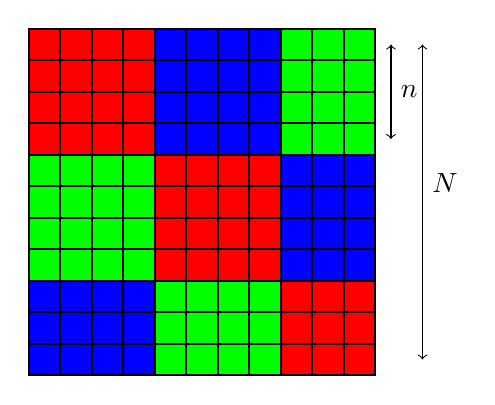
\begin{tikzpicture}
      [%%%%%%%%%%%%%%%%%%%%%%%%%%%%%%
          box/.style={rectangle,draw=black,thick, minimum size=.4cm},
          scale=0.4
      ]%%%%%%%%%%%%%%%%%%%%%%%%%%%%%%

  \foreach \x in {0,1,...,10}{
      \foreach \y in {0,1,...,10}
          \node[box] at (\x,\y){};
  }

  \foreach \x in {0,...,3}{
      \foreach \y in {7,...,10}
        \node[box,fill=red] at (\x,\y){};
  }

  \foreach \x in {4,...,7}{
      \foreach \y in {7,...,10}
        \node[box,fill=blue] at (\x,\y){};
  }

  \foreach \x in {8,...,10}{
      \foreach \y in {7,...,10}
        \node[box,fill=green] at (\x,\y){};
  }

  \foreach \x in {0,...,3}{
      \foreach \y in {3,...,6}
        \node[box,fill=green] at (\x,\y){};
  }

  \foreach \x in {4,...,7}{
      \foreach \y in {3,...,6}
        \node[box,fill=red] at (\x,\y){};
  }

  \foreach \x in {8,...,10}{
      \foreach \y in {3,...,6}
        \node[box,fill=blue] at (\x,\y){};
  }

  \foreach \x in {0,...,3}{
      \foreach \y in {0,...,2}
        \node[box,fill=blue] at (\x,\y){};
  }

  \foreach \x in {4,...,7}{
      \foreach \y in {0,...,2}
        \node[box,fill=green] at (\x,\y){};
  }

  \foreach \x in {8,...,10}{
      \foreach \y in {0,...,2}
        \node[box,fill=red] at (\x,\y){};
  }

  \draw[<->] (11,7) -- (11,10);
  \node[anchor=south west] at (11,8) {$n$};
  \draw[<->] (12,0) -- (12,10);
  \node[anchor=south west] at (12,5) {$N$};

  \end{tikzpicture}
\end{wrapfigure}

\noindent There is also research into applying loop tiling to the generated code, which is dividing the iterations of a loop into sub-regions where both temporal and spatial locality in memory can be exploited.\\
For example, a loop iterating over a 2D array of size $N \times N$, with Level 1 (L1) cache size of $n$ such that $n < N$ would benefit from dividing the array into squares of size at most $n \times n$, as long as this does not violate any data dependencies in the order of operations (see Figure \ref{fig:tile2D}). Doing so prevents values from being evicted from L1 cache prior to being needed again.
\par
Currently this has only been applied to OPS \cite{opstiling}, the precursor to OP2 \cite{opsmain}, which supports structured mesh solvers only. There does exist a 2019 paper \cite{slope} on automated loop tiling for unstructed meshes, and the issues posed by the need for indirect array accesses. A library provided which demonstrates the technique \cite{SLOPErep}, including a demo using the same \textit{airfoil} application used for this report.
\par
During this project it was suggested that applying loop tiling inside the JIT compilation stage could be a good extension, and would likely provide speedup, however unfortunately there was not sufficient time to reasonably expect the functionality to be finished.

\subsubsection{CUDA JIT Compilation}
Going in a different direction, the CUDA library does provide an interface for JIT compilation natively, which would allow for re-compilation without requiring a system call to \verb|make| for every loop kernel. System calls can be a significant bottleneck in some cases, and this problem would only compound for applications with a large number of parallel loops. Therefore, using the CUDA JIT compilation system would likely bring down the upfront cost of recompilation. For \textit{airfoil} this re-compile time is very low, it would not have much impact on the results gathered.

\subsubsection{Alternative Hardware Targets}
Finally, there are other hardware targets supported by OP2 which may be able to benefit from Just-In-Time compilation, and since the purpose of OP2 is to provide performance on multiple hardware platforms from a single application code any new optimisation which is found to improve performance, should also be ported to other platforms where it might be able to provide benefit. Any users who do not  primarly utilise Nvidia GPU hardware should benefit from the JIT compilation optimisation.

\subsection{Project Management}
\label{ss:pm}
